
\documentclass[ms.tex]{subfiles}
\begin{document}

\section{Application to the H3 Survey}
\label{sec:h3}

\begin{itemize}

	\item Next we apply our fitting method to two dwarf satellite remnants
	observed in the Milky Way halo: the Gaia-Sausage Enceladus (GSE) and the
	Sagittarius (Sgr) dwarf Spheroidal (dSph).
	We choose these systems because they probe two qualitatively different SFHs.
	The GSE exhibits smooth, monotonic trends of~\afe~with~\feh~(see
	Fig.~\ref{fig:gse_bestfit} and discussion in~\S~\ref{sec:h3:gse} below),
	an empirical result which does not demand a sudden event such as a
	starburst in its explanation.
	The Sgr dSph, on the other hand, exhibits an increase in~\afe~which is
	accompanied by an increase in the observed density of stars (see
	Fig. X and discussion in~\S~\ref{sec:h3:sgr} below).
	This result, contrary to the GSE data, is naturally explained by a burst in
	star formation.

\end{itemize}

\subsection{The H3 Survey}
\label{sec:h3:survey}

\subsection{The Gaia-Sausage Enceladus}
\label{sec:h3:gse}

\begin{figure*}
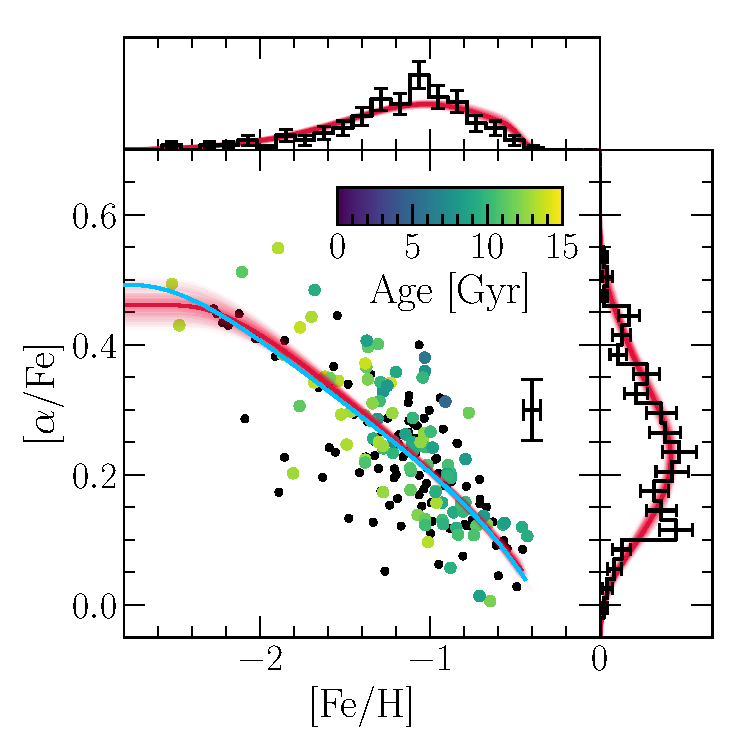
\includegraphics[scale = 0.5]{gsefit_afe_feh.pdf}
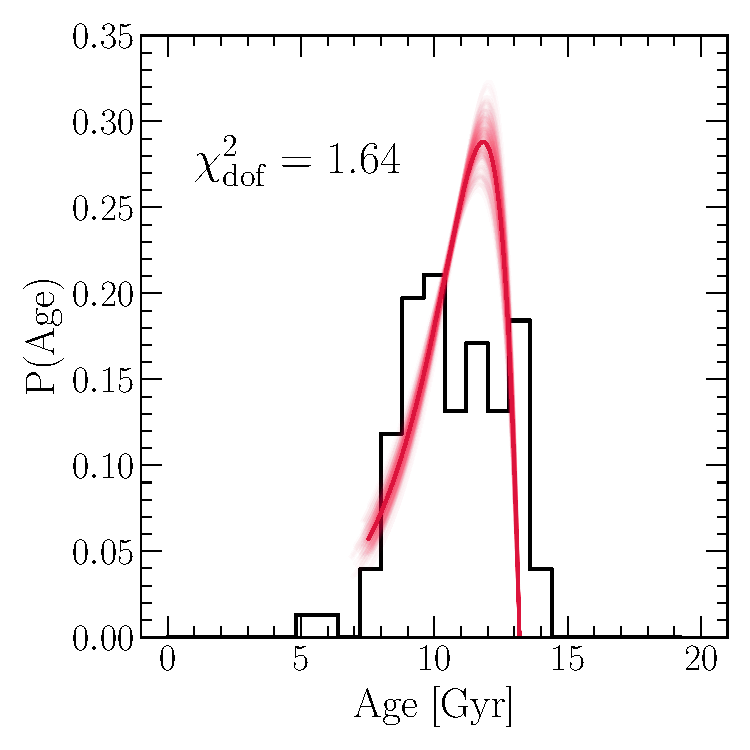
\includegraphics[scale = 0.42]{gsefit_agedist.pdf}
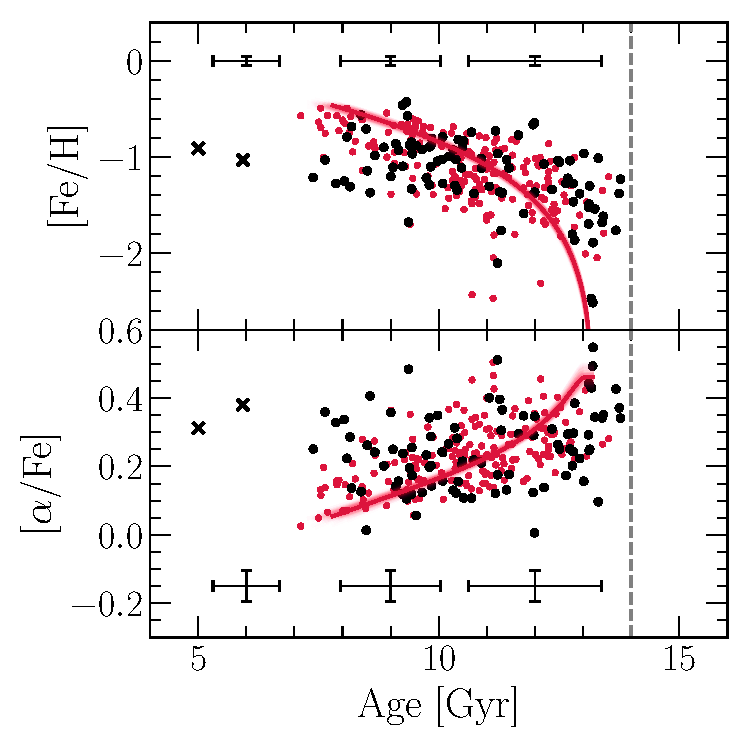
\includegraphics[scale = 0.42]{gsefit_amr.pdf}
\caption{Our fit to the GSE data observed by the H3 survey.}
\label{fig:gse_bestfit}
\end{figure*}

\begin{figure*}
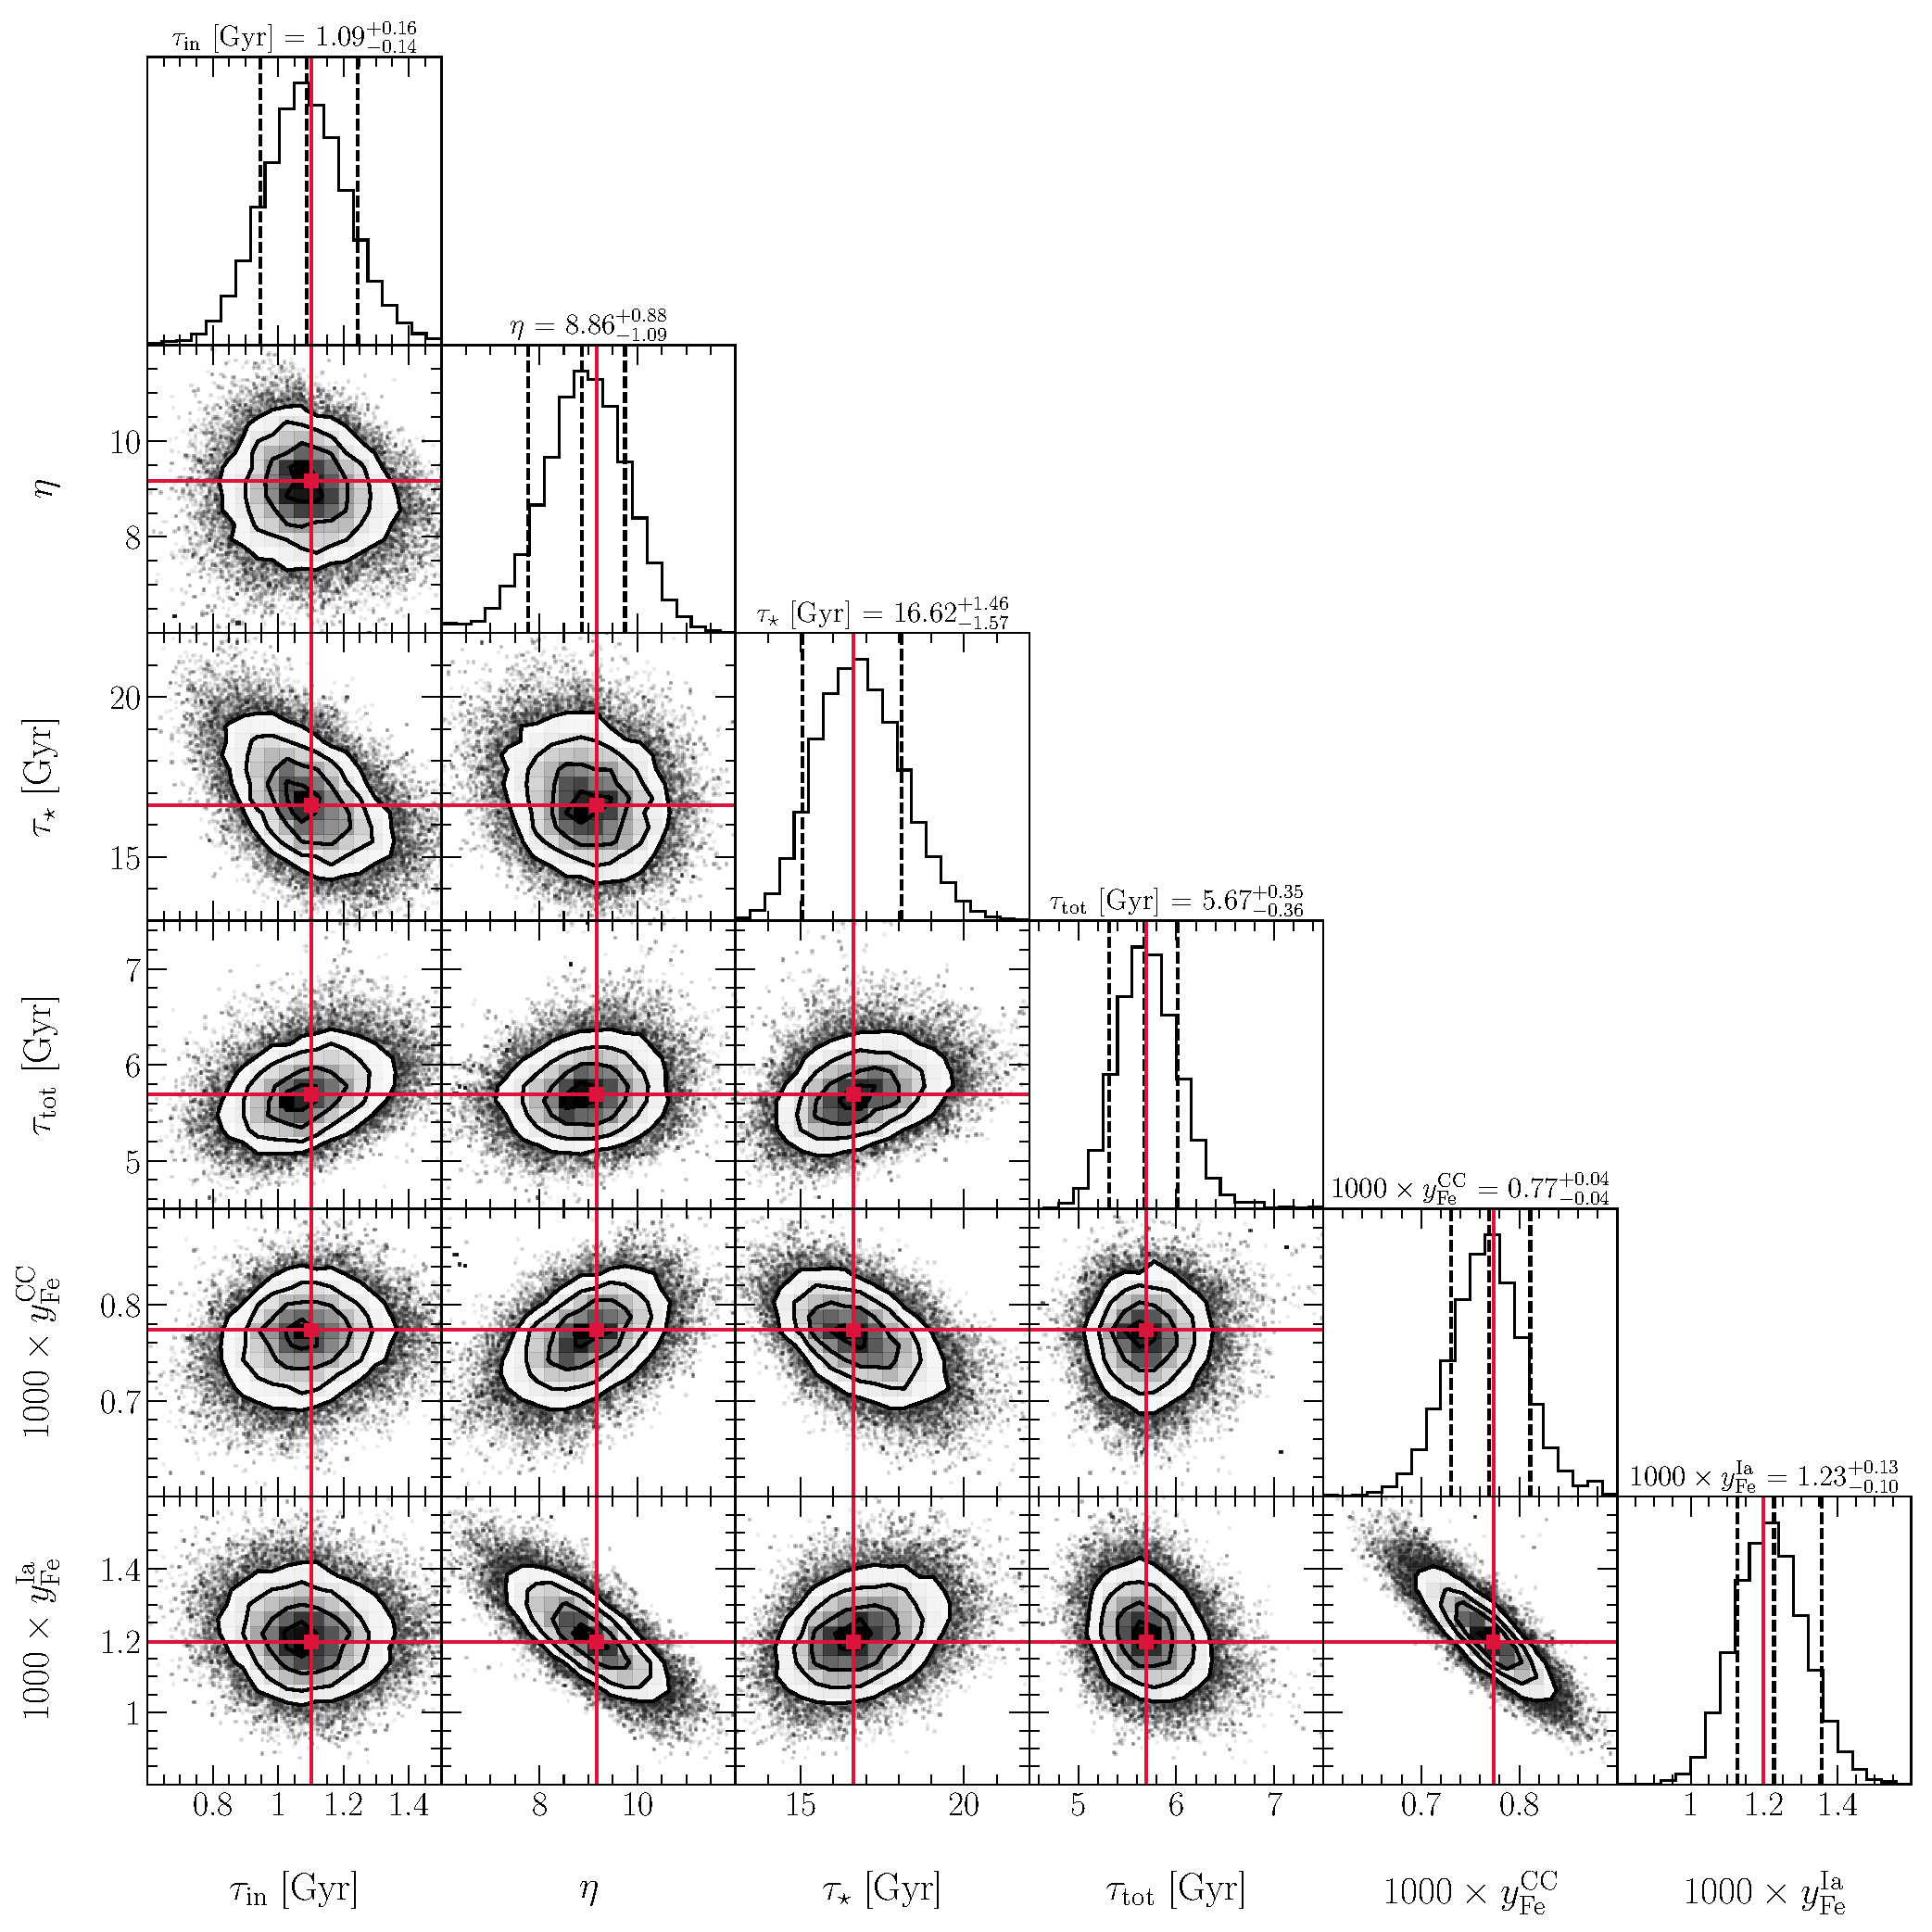
\includegraphics[scale = 0.45]{gsechem_102k4.pdf}
\caption{The ``corner-plot`` showing the results of our fitting method
applied to GSE stars observed by the H3 survey.}
\label{fig:gse_corner}
\end{figure*}

\subsection{The Sagittarius Dwarf Spheroidal}
\label{sec:h3:sgr}

\end{document}

